\documentclass[final]{beamer}

\usepackage[orientation=landscape, size=a1, scale=1.4, debug]{beamerposter}
\usepackage{booktabs}
\usepackage{dcolumn}
\usepackage{colortbl}
\usepackage{xcolor}
\usepackage{hyperref}
\usepackage{amsmath}
%\usepackage[absolute, showboxes, overlay]{textpos}
\usepackage[absolute, overlay]{textpos}
\usepackage{calc}
%\usepackage[colorgrid,texcoord]{eso-pic}
\usepackage[bibstyle=numeric,maxcitenames=6]{biblatex}

% \defaultfontfeatures{Mapping=tex-text}
\usepackage{pifont}
\usepackage{multicol}
\usepackage{algorithm}
\usepackage[noend]{algpseudocode} 
\usepackage{mathtools}
\usepackage{array}
\usepackage{color}
\usepackage[export]{adjustbox}
\usepackage{multirow}
\usepackage{dsfont}
\usepackage{bm}
\usepackage{xcolor}

% \newcolumntype{L}[1]{>{\raggedright\let\newline\\\arraybackslash\hspace{0pt}}m{#1}}
% \newcolumntype{C}[1]{>{\centering\let\newline\\\arraybackslash\hspace{0pt}}m{#1}}
% \newcolumntype{R}[1]{>{\raggedleft\let\newline\\\arraybackslash\hspace{0pt}}m{#1}}

\usetheme{enziteto}

\addbibresource{../referomnia/referomnia.bib}

\usepackage{blindtext}

% \newcommand*\mccol[2]{\multicolumn{#1}{c}{#2}}
% \newcommand*\tmccol[2]{\mccol{#1}{\tiny\textsf{#2}}}
% \newcommand*\bmccol[2]{\mccol{#1}{\textbf{#2}}}
\newcommand{\argmax}{\operatornamewithlimits{argmax}}
\newcommand{\argmin}{\operatornamewithlimits{argmin}}
\newcommand{\nodeset}[1]{\bm{\mathsf{#1}}}

\definecolor{lacamgreen} {RGB} {72, 175, 115}
\definecolor{lacamlilac} {RGB} {107,93,153}
\definecolor{lacamlilac2} {RGB} {93, 109, 152}
\definecolor{lacamlightlilac} {RGB} {174, 166, 201}
\definecolor{lacamdarklilac} {RGB} {51, 10, 102}
\definecolor{lacamgold} {RGB} {255, 87, 0}
\definecolor{lacamdarklilac5} {RGB} {51, 10, 102}
\definecolor{lacamgold5} {RGB} {255, 87, 0}
\definecolor{violet} {RGB} {119, 111, 178}
\definecolor{petroil2} {RGB} {36, 165, 175}
\definecolor{petroil4} {RGB} {30, 132, 149}
\definecolor{petroil6} {RGB} {23, 101, 115}
\definecolor{gold2} {RGB} {255, 130, 0}
\definecolor{gold4} {RGB} {250, 100, 0}
\definecolor{gold6} {RGB} {245, 90, 0}

\newcommand{\highlight}[2][yellow]{\mathchoice%
  {\colorbox{#1}{\strut\textcolor{white}{$\displaystyle{#2}$}}}%
  {\colorbox{#1}{\strut\textcolor{white}{$\textstyle{#2}$}}}%
  {\colorbox{#1}{\strut\textcolor{white}{$\scriptstyle{#2}$}}}%
  {\colorbox{#1}{\strut\textcolor{white}{$\scriptscriptstyle{#2}$}}}}%

\newcommand{\highlighttext}[2][yellow]{{\colorbox{#1}{\strut\textcolor{white}{#2}}}}


\def\restrict#1{\mkern 1mu \vrule height 1.3ex\mkern2mu #1}

\makeatletter
\def\maketag@@@#1{\hbox{\m@th\normalfont\small#1}\hspace{30pt}}
\makeatother


\newcolumntype{R}[2]{
  >{\adjustbox{angle=#1,lap=\width-(#2)}\bgroup}
  l
  <{\egroup}
}

\newcommand*\rot{\multicolumn{1}{R{45}{1em}}}
% \newcommand*\rot{\rotatebox{60}}

% 
% custom colors
\definecolor{untractable_red}{RGB}{209, 25, 25}
\definecolor{tractable_green}{RGB}{0, 153, 51}

\newcommand{\cmark}{\ding{51}}%
\newcommand{\xmark}{\ding{55}}

\newcommand{\summark}{\tiny\textcolor{lacamlilac}{$\boldsymbol{\oplus}$}}
\newcommand{\prodmark}{\tiny\textcolor{lacamlilac}{$\boldsymbol{\otimes}$}}

\setbeamertemplate{itemize item}{\raisebox{.21ex}{\hbox{\summark}\hspace{0pt}}}
\setbeamertemplate{itemize subitem}{\raise .2ex\hbox{\prodmark}\hspace{0pt}}
\setbeamertemplate{itemize subsubitem}{\textcolor{lacamlilac}{$\oplus$}}
% \setbeamertemplate{bibliography item}{\hspace{10pt}\raise
%   .2ex\hbox{\tiny\textcolor{lacamlilac}{$\boldsymbol{\oplus}$}}\insertbiblabel}
\setbeamertemplate{bibliography item}{\insertbiblabel}


\setbeamertemplate{headline}{}

% \addbibresource{../referomnia/referomnia.bib}

\title{Fast and Accurate Denstiy Estimation with Extremely Randomized
  Cutset Networks}
\author{Nicola  {Di Mauro}, Antonio  Vergari, Teresa M.A. Basile and Floriana Esposito}
\date{}


\begin{document}

\institute{Università degli Studi di Bari}
% \department{Dipartimento di Informatica}
% \laboratory{LACAM}
% \group{Machine Learning}

% \institutelogo{
\includegraphics[width=25pt]{figures/unibaba}}
% \lablogo{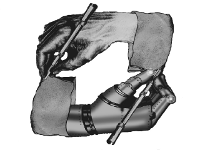
\includegraphics[width=35pt]{figures/lacam}}


% {
%   \setbeamertemplate{headline}{}
%   \setbeamertemplate{footline}{}
%   \begin{textblock}
%     \titlepage
%   \end{textblock}
% }

\newcommand{\hmargin}{25mm}
\newcommand{\vmargin}{30mm}
\textblockorigin{\hmargin}{\vmargin}

\setlength{\TPHorizModule}{1cm}
\setlength{\TPVertModule}{1cm}

%
% TODO: generalize this
\newlength{\posterwidth}
\newlength{\posterheight}
\setlength{\posterwidth}{1189mm}
\setlength{\posterheight}{841mm - 2\hmargin}

\newcommand{\ncols}{3}
\newcommand{\scalefactor}{1.4}
\newlength{\colwidth}
\setlength{\colwidth}{\posterwidth/\ncols}

\newlength{\colhpoint}
\setlength{\leftmargini}{35pt}


\begin{frame}{}
  %
  % title
  % \textblockcolour{header}
  \begin{textblock}{78}(0, 0)
    \usebeamerfont{section name}
    \Huge
    Fast and Accurate Density Estimation with\\
    Extremely Randomized Cutset Networks
  \end{textblock}
  %
  % authors
  \begin{textblock}{40}(50, 0.3)
    \usebeamerfont{author}
    \small
    Nicola {Di Mauro}${}^{\text{\summark}}$\\[10pt]
    Antonio Vergari${}^{\text{\summark}}$\\[10pt]
    Teresa M. A. Basile${}^{\text{\prodmark}}$\\[10pt]
    Floriana Esposito${}^{\text{\summark}}$
  \end{textblock}
  % 
  % email
  \begin{textblock}{7}(51, 0.5)
    %\usebeamerfont{author}
    \scriptsize
    \flushright
    \emph{nicola.dimauro@uniba.it}\\[19pt]
    \emph{antonio.vergari@uniba.it}\\[17pt]
    \emph{teresamaria.basile@uniba.it}\\[17pt]
    \emph{floriana.esposito@uniba.it}
  \end{textblock}
  %
  % affiliations
    \begin{textblock}{30}(60, 0)
    \usebeamerfont{author}
    \scriptsize
    \begin{minipage}[t]{20cm}
      \vspace{0pt}\hspace{15pt}
      
\includegraphics[width=95pt]{figures/unibaba}
      \hspace{10pt}
      \vspace{5pt}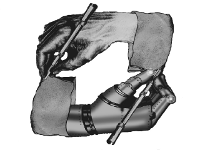
\includegraphics[width=140pt]{figures/lacam}
      \hspace{10pt}
      
\includegraphics[width=90pt]{figures/infn}
      \hspace{10pt}
      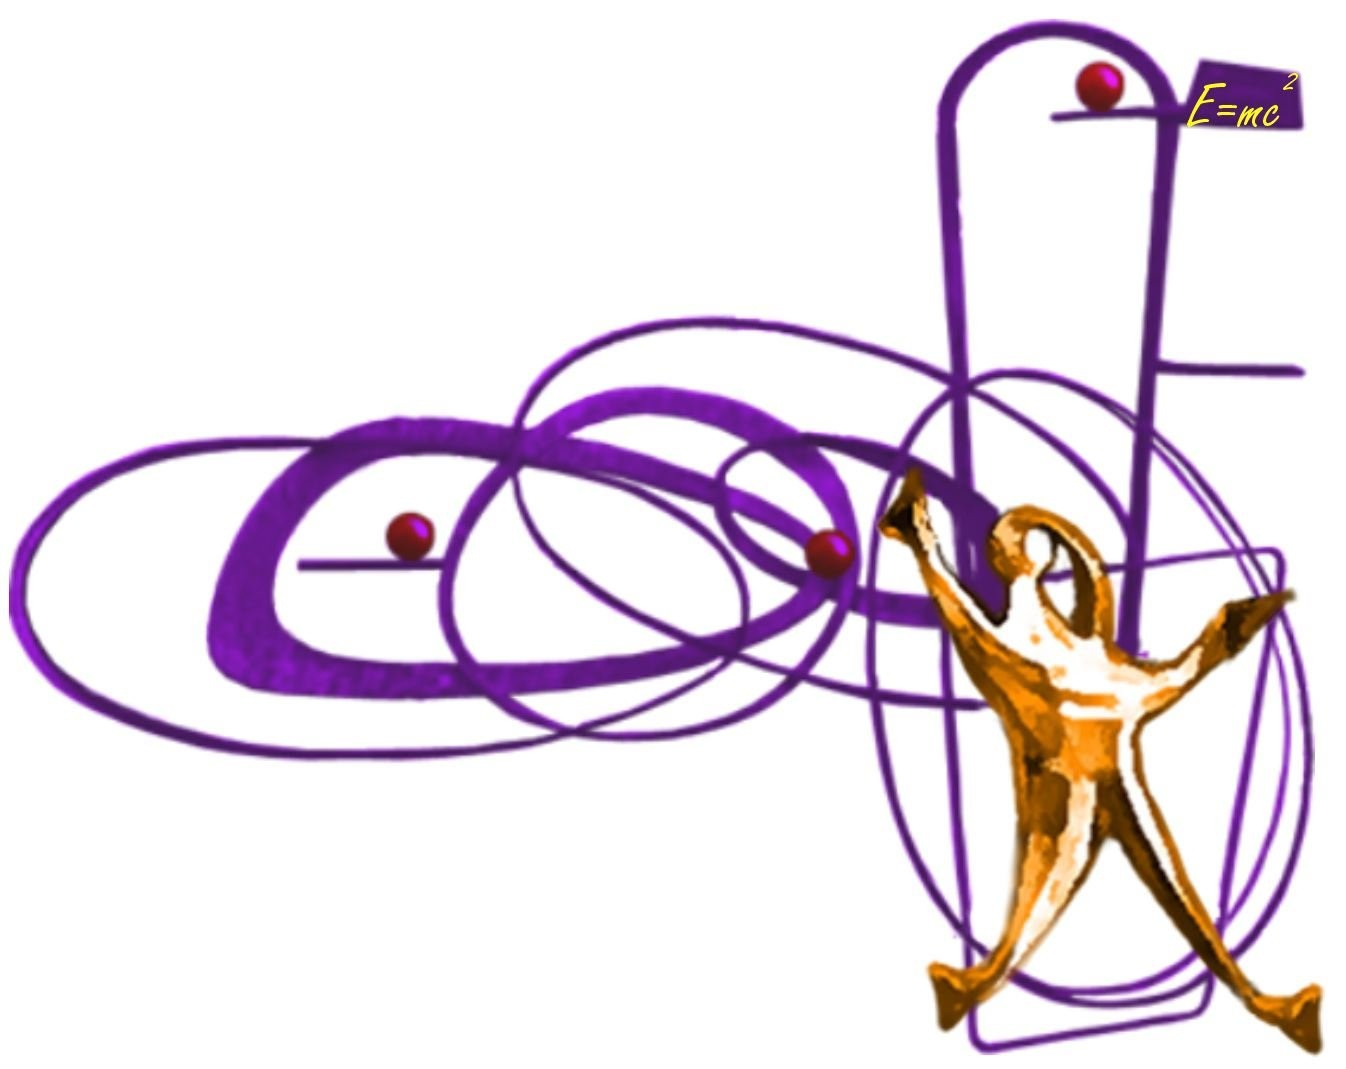
\includegraphics[width=130pt]{figures/fisicalogo}
    \end{minipage}\hspace{-5pt}
    \begin{minipage}[t]{15cm}
    \vspace{30pt}
      
    \end{minipage}
  \end{textblock}
  % \begin{textblock}{30}(55, 0)
  %   \usebeamerfont{author}
  %   \scriptsize
  %   \begin{minipage}[t]{5cm}
  %     \vspace{0pt}\hspace{15pt}
  %     
\includegraphics[width=110pt]{figures/unibaba}
  %   \end{minipage}\hspace{-5pt}
  %   \begin{minipage}[t]{15cm}
  %   \vspace{30pt}
  %     \flushleft
  %     % University of Bari, Italy\\
  %     University of Bari\\
  %   \vspace{2pt}
  %   % Computer Science Department
  %   LACAM - Machine Learning
  %   \end{minipage}\\[0.75cm]
  %   \usebeamerfont{author}
  %   \scriptsize
  %   \begin{minipage}[t]{5cm}
  %     \vspace{-5pt}
  %     % 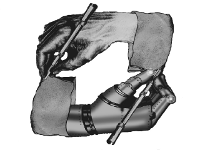
\includegraphics[width=145pt]{figures/lacam}
  %     %\hspace{28pt}\includegraphics[width=95pt]{figures/cam-logo-big-gray.png}
  %   \end{minipage}\hspace{-5pt}
  %   \begin{minipage}[t]{15cm}
  %     \vspace{20pt}
  %     \flushleft
  %     % LACAM Laboratory\\
  %     University of Cambridge\\
  %     \vspace{2pt}
  %     % Machine Learning
  %     Department of Engineering
  %   \end{minipage}
  % \end{textblock}
  
  
  %
  % column I
  \begin{textblock}{17.5}(0, 7)
    \usebeamerfont{section name}
    1. Density estimation
  \end{textblock}

  \begin{textblock}{17.5}(0, 8.7)
    \small
    % \blindtext
        \emph{\textbf{Density estimation}} is the unsupervised task of
    learning an estimator for the joint probability distribution
    $p(\mathbf{X})$ from a set of i.i.d. samples $\mathcal{D}=\{\mathbf
    x^i\}_{i=1}^m$ over r.v.s $\mathbf{X}=\{X_{1},\dots,X_{n}\}$\\[20pt]
    
    Given such an estimator, one uses it to answers
    probabilistic queries about configurations on $\mathbf{X}$,
    i.e. to do \emph{\textbf{inference}}.\\[20pt]

    The main challenge in density estimation is balancing:
    \begin{itemize}
    \item the \highlighttext[lacamlightlilac]{\textbf{\emph{representation expressiveness}}} of a model
    \item the \highlighttext[lacamlightlilac]{\textbf{\emph{cost of learning}}} it
      \item and the \highlighttext[lacamlightlilac]{\textbf{\emph{cost of performing inference}}} on it.
    \end{itemize}
    

    
    
    % \begin{itemize}
    % \item $p(\mathbf{X} = \mathbf{x})$ pointwise evidence (EVI) 
    % \item $p(\mathbf{E}), \mathbf{E}\subset\mathbf{X}$ marginals (MAR)
    % \item $p(\mathbf{Q}|\mathbf{E}), \mathbf{Q},
    %   \mathbf{E}\subset\mathbf{X}, \mathbf{Q}\cap \mathbf{E}=\emptyset$
    %   conditionals (CON)
    % \item $\arg\max_{\mathbf{q}\sim\mathbf{Q}}p(\mathbf{q}|\mathbf{E})$
    %   MPE assignments (MPE)
    % % \item $Z =\sum_{\mathbf{x}\sim \mathbf{X}}\phi(\mathbf{x})$
    % %   partition function (Z)
    %   \item sampling: generate $\mathbf{x}\sim p(\mathbf{X})$ (SAM)
    % \end{itemize}\vspace{20pt}

  \end{textblock}

  \begin{textblock}{17.5}(0, 20)
    \usebeamerfont{section name}
    %\normalsize
    2. Tractable Probabilistic Models (TPMs)
  \end{textblock}
  
  \begin{textblock}{17.5}(0, 23.4)
    \small

    Classical Probabilistic Graphical Models like \emph{\textbf{Bayesian Networks}}
    (\textbf{BNs}) and \emph{\textbf{Markov Networks}} (\textbf{MNs}) are highly expressive but
    exact inference is generally NP-hard~\cite{Roth1996}.
    \vspace{20pt}

    
    \emph{\textbf{Tractable Probabilistic Models} }  (\textbf{TPMs})
    on the other hand, are density estimators for which some kind of  \textbf{\emph{exact}} inference is
    \textbf{\emph{tractable}}, i.e. \emph{polynomial} in the number of RVs or their
    domains.
    \hfill$\rightarrow$ Learning them may still be hard to scale.\\[20pt]

    
    {\bf 2.1 Product of Bernoullis (PoBs)}
    The least expressive, assuming all RVs to be independent:
    
    $$\highlight[lacamlightlilac]{\mathsf{p}(\mathbf{x}) =\prod\nolimits_{i=1}^{n}\mathsf{p}(x_{i})}$$

    Learning a PoB has linear time complexity $O(nm)$.\par
    Inference is linear as well, $O(n)$.
    \vspace{20pt}

    {\bf 2.2 Chow-Liu Trees (CLTrees)}

    A \emph{directed tree-structured model}~\cite{Meila2000} over
    $\mathbf{X}$ is a BN in which each node $X_{i}\in\mathbf{X}$ has at most one
    parent, $\mathrm{Pa}_{X_i}$.

    $$\highlight[lacamlightlilac]{\mathsf{p}(\mathbf{x}) =
    \prod\nolimits_{i=1}^n\mathsf{p}(x_i|\mathrm{Pa}_{x_i})}$$

    Learning a \textsf{CLtree} takes  quadratic time $O(n^2(m + \log n))$.\par
    Inference is still linear like \textsf{PoBs}, $O(n)$.
  \end{textblock}

  % \begin{textblock}{17.5}(0, 33)
  %   \usebeamerfont{section name}
  %   3. Density estimation
  % \end{textblock}
  
  % \begin{textblock}{17.5}(0, 34.7)
  %   \small
  %   \blindtext
  % \end{textblock}

  %
  % column 2
  \begin{textblock}{17.5}(20.5, 7)
    \usebeamerfont{section name}
    3. Cutset Networks (CNets)
  \end{textblock}
  
  \begin{textblock}{17.5}(20.5, 8.7)
    \small

    A Cutset Network (CNet) $\mathcal{C}$ is TPM represented via a
    weighted probabilistic model tree over $\mathbf{X}$ and
    recursively defined as:
    \begin{enumerate}
    \item a TPM $\mathcal{M}$, with
      $\mathsf{scope}(\mathcal{M})=\mathbf X$
      \item a weighted  disjunction (OR node) of two CNets $\mathcal C_0$ and $\mathcal C_1$
     conditioned on RV $X_i \in \mathbf X$,  with
    weights $w_i^0$ and $w_i^1$ s.t. $w_i^0 + w_i^1 = 1$,
    where $\mathsf{scope}(\mathcal C_{0})=\mathsf{scope}(\mathcal C_{1})=\mathbf X_{\setminus i}$
    \end{enumerate}
    \begin{figure}
     \centering
     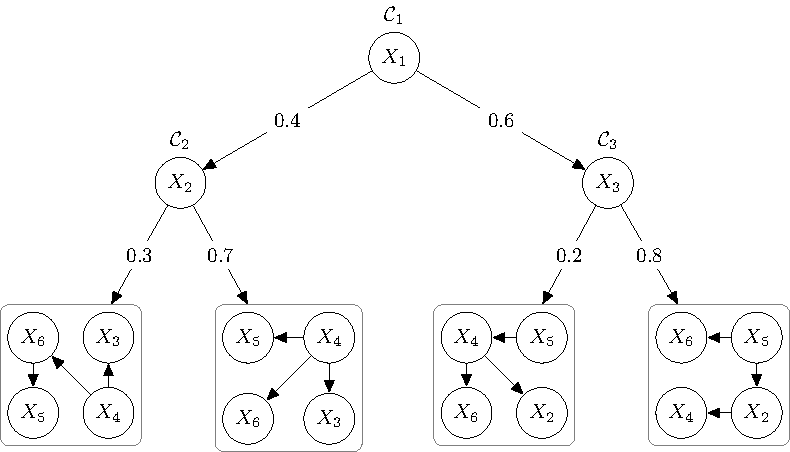
\includegraphics[width=15cm]{figures/csn}
     % \caption{\scriptsize }
  \label{fig:csn}
\end{figure}
\hspace{50pt}
\begin{minipage}{0.8\linewidth}
\scriptsize  A CNet over binary RVs
$\mathbf{X}=\{X_1,\dots,X_{6}\}$. Or nodes are rounded, while leaf squared nodes represent CLtrees.
\end{minipage}

\vspace{20pt}
Therefore, the joint pdf modeled by a CNet $\mathcal{C}$ is:
\begin{equation}
\highlight[lacamlightlilac]{\mathsf{p}(\mathbf{x}) = \mathsf{p}_l(\mathbf
x_{|\mathsf{scope}(\mathcal C)\setminus \mathsf{scope}(\mathcal
  M_l)})\mathsf{p}_{\mathcal M_l}(\mathbf x_{| \mathsf{scope}(\mathcal
  M_l)})}\label{eq:cnetdistr}
\end{equation}


  \end{textblock}

  \begin{textblock}{17.5}(20.5, 29.5)
    \usebeamerfont{section name}
    4. Learning CNets
  \end{textblock}
  
  \begin{textblock}{17.5}(20.5, 31.2)
  % \begin{textblock}{17.5}(20.5, 20)
  %   \usebeamerfont{section name}
  %   2. Learning CNets
  % \end{textblock}
  % \begin{textblock}{17.5}(20.5, 21.7)
    \small
    
    All top-down greedy CNet learners %~\cite{Rahman2014,DiMauro2015a}
    can be unified in single template, $\mathsf{LearnCNet}$:
 \begin{center}  
  \begin{minipage}{0.9\linewidth}
    \vspace{10pt}
        \scriptsize
        {\hrule\flushleft\textsf{LearnCNet}($\mathcal{D}$, $\mathbf{X}$, $\alpha$,
        $\delta$, $\sigma$)\\\hrule}
        % \blindtext
%\begin{algorithm}
%  \caption{\textsf{\textsf{LearnCNet}}($\mathcal{D}$, $\mathbf{X}$, $\alpha$, $\delta$, $\sigma$)}
%  \label{algo:learn-cnet}
  \begin{algorithmic}[1]
    \State \textbf{Input:} a dataset $\mathcal{D}$ over RVs $\mathbf{X}$; $\alpha$: $\delta$
    min number samples; $\sigma$ min number features
    \State  \textbf{Output:}  a CNet $\mathcal{C}$ encoding  $\mathsf{p}_{\mathcal{C}}(\textbf{X})$ learned from $\mathcal D$
    \If {$|\mathcal D|>\delta$ \textbf{and} $|\mathbf X|>\sigma$}
    \State $\highlight[lacamlightlilac]{X_i\leftarrow  \mathsf{select}(\mathcal D, \mathbf X, \alpha)}$
    % \If {$\mathsf{success}$}
    \Comment {select the RV to condition on}
    \State $\mathcal D_0 \leftarrow \{\xi \in \mathcal D: \xi[X_i]=0 \}$, $\mathcal D_1 \leftarrow \{\xi \in \mathcal D: \xi[X_i]=1 \}$
    \State $w_0 \leftarrow |\mathcal D_0| / |\mathcal D|$, $w_1 \leftarrow |\mathcal   D_1| / |\mathcal D|$
    \State $\mathcal{C} \leftarrow
    w_0\cdot\mathsf{LearnCNet}(\mathcal D_0, \mathbf X_{\setminus i},
    \alpha, \delta, \sigma) + w_1 \cdot\mathsf{LearnCNet}(\mathcal D_1, \mathbf X_{\setminus i}, \alpha, \delta, \sigma) $
    % \Else 
    % \State $C \leftarrow \mathcal T$ 
    %\EndIf
    \Else 
    \State $\mathcal{C} \leftarrow \mathsf{learnLeafDistribution}(\mathcal D, \mathbf X, \alpha)$
    \EndIf
    \State \Return $\mathcal{C}$
  \end{algorithmic}
  \hrule
  
\end{minipage}
\end{center}
\vspace{10pt}
    different \highlighttext[lacamlightlilac]{\textsf{select} implementations}
    have different complexities:
    \vspace{10pt}

    \begin{center}
      \begin{minipage}{0.9\linewidth}
        \begin{description}[align=parright]
        \item[\textbf{\textsf{entCNet}}~\cite{Rahman2014}] choosing
          $X_{i}$ to lower approximate average joint entropy
          {\hfill $\rightarrow\highlight[lacamlightlilac]{O(mn^2)}$}
        \item[\textbf{\textsf{dCSN}}~\cite{DiMauro2015a}] choosing
          $X_{i}$ in a principled way improving likelihood
          {\hfill $\rightarrow$ $\highlight[lacamlightlilac]{O(n^3(m + \log n))}$}
        \end{description}
      \end{minipage}
    \end{center}
    
  \end{textblock}

  % \begin{textblock}{17.5}(20.5, 33)
  %   \usebeamerfont{section name}
  %   2. Cutset Networks
  % \end{textblock}

  % \begin{textblock}{17.5}(20.5, 34.7)
  %   \small
  %   \blindtext
  % \end{textblock}


  %
  % column 3

  \begin{textblock}{17.5}(41, 7)
    \usebeamerfont{section name}
    5. XCNets
  \end{textblock}
  \begin{textblock}{17.5}(41, 8.7)
    \small
    \emph{\textbf{XCNets}} (\textbf{Extremely Randomized CNets}) are CNets built by \textsf{LearnCNet} when
    \textsf{select} chooses one RV \emph{completely at random}.\par
    {\hfill\textsf{select} time complexity $\rightarrow$ $\highlight[lacamlightlilac]{O(1)}$!}
    \vspace{20pt}


    {\bf 5.1 Mixture of Experts Interpretation}\par
    A single CNet can be seen as a peculiar \emph{mixture of experts}: the OR
    tree plays as a \emph{deterministic gating function} and leaf distributions
    as \emph{local experts}.
    A path $p=p_{(1)}p_{(2)}\cdots p_{(k)}$ connects the root to a
    single leaf $\mathcal{M}_{l}$ after observing $x_{1} x_{2} \cdots  x_{k}$,
     Equation~\ref{eq:cnetdistr}.

$\mathsf{p}_l(\mathbf x_{|\mathsf{sc}(\mathcal C)\setminus
  \mathsf{sc}(\mathcal M_l)})$ is decomposed by the chain rule across
path $p$ .\par
{\hfill$\rightarrow$ randomly shuffling
  $X_{p_(0)},\dots,X_{p_{k}}$ does not influence inference!}

\vspace{20pt}
Therefore a single \textsf{XCNet} is only only slightly less accurate
than a \textsf{CNet} and as good at generating samples.

    
    % Other advantages of XCNets are comparable or only slightly less accurate as density estimators that
    % CNets learned by $dCSN$ (see Exp 4.1)
    % and as good as sample generators.
    % \vspace{10pt}

    \begin{figure}[t]
  \centering
  \setlength{\tabcolsep}{0pt}
  \renewcommand{\arraystretch}{0}
  \newcolumntype{S}{>{\centering\arraybackslash} m{.045\linewidth} }
  \newcolumntype{X}{>{\centering\arraybackslash} m{.03\linewidth} }
\begin{tabular}{SSSSSXSSSSSXSSSSSXSSSSS}
 
\includegraphics[width=\linewidth]{{figures/mnist.cnet.50.0}.pdf}
& 
\includegraphics[width=\linewidth]{{figures/mnist.cnet.50.1}.pdf}
& 
\includegraphics[width=\linewidth]{{figures/mnist.cnet.50.2}.pdf}
& 
\includegraphics[width=\linewidth]{{figures/mnist.cnet.50.3}.pdf}
& 
\includegraphics[width=\linewidth]{{figures/mnist.cnet.50.5}.pdf}
&
& 
\includegraphics[width=\linewidth]{{figures/mnist.cnet.near.50.0}.pdf}
& 
\includegraphics[width=\linewidth]{{figures/mnist.cnet.near.50.1}.pdf}
& 
\includegraphics[width=\linewidth]{{figures/mnist.cnet.near.50.2}.pdf}
& 
\includegraphics[width=\linewidth]{{figures/mnist.cnet.near.50.3}.pdf}
& 
\includegraphics[width=\linewidth]{{figures/mnist.cnet.near.50.5}.pdf}
&    
& 
\includegraphics[width=\linewidth]{{figures/mnist.xcnet.50.1}.pdf}
& 
\includegraphics[width=\linewidth]{{figures/mnist.xcnet.50.2}.pdf}
& 
\includegraphics[width=\linewidth]{{figures/mnist.xcnet.50.3}.pdf}
& 
\includegraphics[width=\linewidth]{{figures/mnist.xcnet.50.4}.pdf}
& 
\includegraphics[width=\linewidth]{{figures/mnist.xcnet.50.5}.pdf}
&
& 
\includegraphics[width=\linewidth]{{figures/mnist.xcnet.near.50.1}.pdf}
& 
\includegraphics[width=\linewidth]{{figures/mnist.xcnet.near.50.2}.pdf}
& 
\includegraphics[width=\linewidth]{{figures/mnist.xcnet.near.50.3}.pdf}
& 
\includegraphics[width=\linewidth]{{figures/mnist.xcnet.near.50.4}.pdf}
& 
\includegraphics[width=\linewidth]{{figures/mnist.xcnet.near.50.5}.pdf}\\

 
\includegraphics[width=\linewidth]{{figures/mnist.cnet.50.6}.pdf}
& 
\includegraphics[width=\linewidth]{{figures/mnist.cnet.50.7}.pdf}
& 
\includegraphics[width=\linewidth]{{figures/mnist.cnet.50.8}.pdf}
& 
\includegraphics[width=\linewidth]{{figures/mnist.cnet.50.9}.pdf}
& 
\includegraphics[width=\linewidth]{{figures/mnist.cnet.50.11}.pdf}
&
& 
\includegraphics[width=\linewidth]{{figures/mnist.cnet.near.50.6}.pdf}
& 
\includegraphics[width=\linewidth]{{figures/mnist.cnet.near.50.7}.pdf}
& 
\includegraphics[width=\linewidth]{{figures/mnist.cnet.near.50.8}.pdf}
& 
\includegraphics[width=\linewidth]{{figures/mnist.cnet.near.50.9}.pdf}
& 
\includegraphics[width=\linewidth]{{figures/mnist.cnet.near.50.11}.pdf}
&  
& 
\includegraphics[width=\linewidth]{{figures/mnist.xcnet.50.6}.pdf}
& 
\includegraphics[width=\linewidth]{{figures/mnist.xcnet.50.8}.pdf}
& 
\includegraphics[width=\linewidth]{{figures/mnist.xcnet.50.9}.pdf}
& 
\includegraphics[width=\linewidth]{{figures/mnist.xcnet.50.10}.pdf}
& 
\includegraphics[width=\linewidth]{{figures/mnist.xcnet.50.11}.pdf}
&
& 
\includegraphics[width=\linewidth]{{figures/mnist.xcnet.near.50.6}.pdf}
& 
\includegraphics[width=\linewidth]{{figures/mnist.xcnet.near.50.8}.pdf}
& 
\includegraphics[width=\linewidth]{{figures/mnist.xcnet.near.50.9}.pdf}
& 
\includegraphics[width=\linewidth]{{figures/mnist.xcnet.near.50.10}.pdf}
& 
\includegraphics[width=\linewidth]{{figures/mnist.xcnet.near.50.11}.pdf}\\
 
 \includegraphics[width=\linewidth]{{figures/mnist.cnet.50.12}.pdf}
& \includegraphics[width=\linewidth]{{figures/mnist.cnet.50.13}.pdf}
& \includegraphics[width=\linewidth]{{figures/mnist.cnet.50.14}.pdf}
& \includegraphics[width=\linewidth]{{figures/mnist.cnet.50.15}.pdf}
& \includegraphics[width=\linewidth]{{figures/mnist.cnet.50.17}.pdf}
&
& \includegraphics[width=\linewidth]{{figures/mnist.cnet.near.50.12}.pdf}
& \includegraphics[width=\linewidth]{{figures/mnist.cnet.near.50.13}.pdf}
& \includegraphics[width=\linewidth]{{figures/mnist.cnet.near.50.14}.pdf}
& \includegraphics[width=\linewidth]{{figures/mnist.cnet.near.50.15}.pdf}
& \includegraphics[width=\linewidth]{{figures/mnist.cnet.near.50.17}.pdf}
&
&  \includegraphics[width=\linewidth]{{figures/mnist.xcnet.50.12}.pdf}
& \includegraphics[width=\linewidth]{{figures/mnist.xcnet.50.13}.pdf}
& \includegraphics[width=\linewidth]{{figures/mnist.xcnet.50.14}.pdf}
& \includegraphics[width=\linewidth]{{figures/mnist.xcnet.50.16}.pdf}
& \includegraphics[width=\linewidth]{{figures/mnist.xcnet.50.17}.pdf}
&
& \includegraphics[width=\linewidth]{{figures/mnist.xcnet.near.50.12}.pdf}
& \includegraphics[width=\linewidth]{{figures/mnist.xcnet.near.50.13}.pdf}
& \includegraphics[width=\linewidth]{{figures/mnist.xcnet.near.50.14}.pdf}
& \includegraphics[width=\linewidth]{{figures/mnist.xcnet.near.50.16}.pdf}
& \includegraphics[width=\linewidth]{{figures/mnist.xcnet.near.50.17}.pdf}\\

 \includegraphics[width=\linewidth]{{figures/mnist.cnet.50.18}.pdf}
& \includegraphics[width=\linewidth]{{figures/mnist.cnet.50.19}.pdf}
& \includegraphics[width=\linewidth]{{figures/mnist.cnet.50.20}.pdf}
& \includegraphics[width=\linewidth]{{figures/mnist.cnet.50.21}.pdf}
& \includegraphics[width=\linewidth]{{figures/mnist.cnet.50.23}.pdf}
&
& \includegraphics[width=\linewidth]{{figures/mnist.cnet.near.50.18}.pdf}
& \includegraphics[width=\linewidth]{{figures/mnist.cnet.near.50.19}.pdf}
& \includegraphics[width=\linewidth]{{figures/mnist.cnet.near.50.20}.pdf}
& \includegraphics[width=\linewidth]{{figures/mnist.cnet.near.50.21}.pdf}
& \includegraphics[width=\linewidth]{{figures/mnist.cnet.near.50.23}.pdf}
&
& \includegraphics[width=\linewidth]{{figures/mnist.xcnet.50.18}.pdf}
& \includegraphics[width=\linewidth]{{figures/mnist.xcnet.50.19}.pdf}
& \includegraphics[width=\linewidth]{{figures/mnist.xcnet.50.20}.pdf}
& \includegraphics[width=\linewidth]{{figures/mnist.xcnet.50.22}.pdf}
& \includegraphics[width=\linewidth]{{figures/mnist.xcnet.50.23}.pdf}
&
& \includegraphics[width=\linewidth]{{figures/mnist.xcnet.near.50.18}.pdf}
& \includegraphics[width=\linewidth]{{figures/mnist.xcnet.near.50.19}.pdf}
& \includegraphics[width=\linewidth]{{figures/mnist.xcnet.near.50.20}.pdf}
& \includegraphics[width=\linewidth]{{figures/mnist.xcnet.near.50.22}.pdf}
& \includegraphics[width=\linewidth]{{figures/mnist.xcnet.near.50.23}.pdf}\\

 \includegraphics[width=\linewidth]{{figures/mnist.cnet.50.24}.pdf}
& \includegraphics[width=\linewidth]{{figures/mnist.cnet.50.25}.pdf}
& \includegraphics[width=\linewidth]{{figures/mnist.cnet.50.26}.pdf}
& \includegraphics[width=\linewidth]{{figures/mnist.cnet.50.27}.pdf}
& \includegraphics[width=\linewidth]{{figures/mnist.cnet.50.29}.pdf}
&
& \includegraphics[width=\linewidth]{{figures/mnist.cnet.near.50.24}.pdf}
& \includegraphics[width=\linewidth]{{figures/mnist.cnet.near.50.25}.pdf}
& \includegraphics[width=\linewidth]{{figures/mnist.cnet.near.50.26}.pdf}
& \includegraphics[width=\linewidth]{{figures/mnist.cnet.near.50.27}.pdf}
& \includegraphics[width=\linewidth]{{figures/mnist.cnet.near.50.29}.pdf}
&
& \includegraphics[width=\linewidth]{{figures/mnist.xcnet.50.24}.pdf}
& \includegraphics[width=\linewidth]{{figures/mnist.xcnet.50.25}.pdf}
& \includegraphics[width=\linewidth]{{figures/mnist.xcnet.50.26}.pdf}
& \includegraphics[width=\linewidth]{{figures/mnist.xcnet.50.27}.pdf}
& \includegraphics[width=\linewidth]{{figures/mnist.xcnet.50.29}.pdf}
&
& \includegraphics[width=\linewidth]{{figures/mnist.xcnet.near.50.24}.pdf}
& \includegraphics[width=\linewidth]{{figures/mnist.xcnet.near.50.25}.pdf}
& \includegraphics[width=\linewidth]{{figures/mnist.xcnet.near.50.26}.pdf}
& \includegraphics[width=\linewidth]{{figures/mnist.xcnet.near.50.27}.pdf}
& \includegraphics[width=\linewidth]{{figures/mnist.xcnet.near.50.29}.pdf}\\\\\\
&
&\scriptsize (a)
&
&
&
&
&
&\scriptsize (b)
&
&
&
&
&
&\scriptsize (c)
&
&
&
&
&
&\scriptsize (d)\\  

\end{tabular}

% \caption{Samples obtained from a CNet (a), resp. XCNet (c), learned on 
%   samples of the binarized \texttt{MNIST} dataset, and their nearest neighbor in training set (b), resp. (d).} 
\label{fig:vis}
\end{figure}
\hspace{50pt}
\begin{minipage}{0.8\linewidth}
  \vspace{-20pt}
\scriptsize  Samples obtained from a CNet (a), resp. XCNet (c), learned on 
   a binarized version of \texttt{MNIST}, and their nearest neighbor in training set (b), resp. (d).
 \end{minipage}


 \vspace{20pt}
 {\bf 5.2 Regularizing learning}\par
Single CNets learned with $\mathsf{LearnCNet}$ are prone to overfitting, randomization in
 \textsf{XCNets} alleviate this issue
    
\begin{figure}[t]
  %\caption{Negative log-likelihood during learning CNets and XCNets.}
  \label{fig:ll}
  \centering
  \begin{tabular}{ccc}
    \includegraphics[width=0.48\linewidth]{figures/kdd} &
    %\includegraphics[width=0.33\linewidth]{figures/msweb} &
    \includegraphics[width=0.48\linewidth]{figures/tmovie}
  \end{tabular}
\end{figure}
\hspace{50pt}
\begin{minipage}{0.8\linewidth}
  \vspace{-10pt}
\scriptsize  Learning curves of CNets and XCNets (negative
log-likelihoods) on $\mathsf{KddCup2k}$ and $\mathsf{EachMovie}$
The latter overfits much later that the former.
\end{minipage}



\vspace{20pt}
{\bf 5.3 Ensembles} of XCNets do not require to additionally
diversify components and learning up to 500 components is still faster
than learning 40 of other variants:

\vspace{10pt}

    \begin{center}
      \begin{minipage}{0.9\linewidth}
        \begin{description}[align=parright]
        \item[\textbf{\textsf{CNet}}$_{\mathsf{bag}}$]
          bagging \textsf{entCSN}~\cite{Rahman2016a}\par
          %{\hfill $\rightarrow$ $O(mn^2)$}
        \item[\textbf{\textsf{CNet}}$_{\mathsf{boost}}$]
          boosting \textsf{entCSN}~\cite{Rahman2016a}\par
        \item[\textbf{\textsf{dCSN}}$^{k}$]
          bagging \textsf{dCSN}~\cite{DiMauro2015a,DiMauro2015b}\par
        \end{description}
      \end{minipage}
    \end{center}

  \end{textblock}
%   \begin{textblock}{17.5}(41, 22.5)
%     \usebeamerfont{section name}
%     7. Mixture of Experts
%   \end{textblock}
%   \begin{textblock}{17.5}(41, 24.2)
%     \small
%     A CNet can be seen as \emph{mixture of experts} in which the OR
%     tree plays as a \emph{deterministic gating
% function} and leaf distributions
% act as the \emph{local experts}.

% % \begin{equation}
% % \mathsf{p}(\mathbf{x}) = \mathsf{p}_l(\mathbf x_{|\mathsf{sc}(\mathcal C)\setminus \mathsf{sc}(\mathcal M_l)})\mathsf{p}_{\mathcal M_l}(\mathbf x_{| \mathsf{sc}(\mathcal M_l)}),
% % \label{eq:cnetdistr}
% % \end{equation}

% $\mathsf{p}_l(\mathbf x_{|\mathsf{sc}(\mathcal C)\setminus
%   \mathsf{sc}(\mathcal M_l)})$ is decomposed by the chain rule across
% a path $\mathsf{p}$ going from the root to leaf model
% $\mathcal{M}_{l}$.\par
% {\hfill$\rightarrow$the order of appearance of
%   $X_{\mathsf{p}(0)},\dots,X_{|\mathsf{p}|-1}$ does not change the
%   factorization!}

% % $g(\mathbf{\xi})=\sum_{p\in\mathcal{G}}\prod_{i=1}^{|p|}
% % \mathds{1}\{\xi[X_{p(i)}]=v_{i}\}\mathcal{M}_{p}$
%   \end{textblock}

%   \begin{textblock}{17.5}(41, 34)
%     \usebeamerfont{section name}
%     8. Regularization
%   \end{textblock}
%   \begin{textblock}{17.5}(41, 35.7)
%     \small
%     % \blindtext
%     As a single CNet can be seen as an ensemble,
%     randomizing the gating function acts as regularization and lessens
%     the overfitting issues with $\mathsf{LearnCNet}$
    
% \begin{figure}[t]
%   %\caption{Negative log-likelihood during learning CNets and XCNets.}
%   \label{fig:ll}
%   \centering
%   \begin{tabular}{ccc}
%     \includegraphics[width=0.48\linewidth]{figures/kdd} &
%     %\includegraphics[width=0.33\linewidth]{figures/msweb} &
%     \includegraphics[width=0.48\linewidth]{figures/tmovie}
%   \end{tabular}
% \end{figure}
% \hspace{50pt}
% \begin{minipage}{0.8\linewidth}
%   \vspace{-10pt}
% \scriptsize  Learning curves of CNets and XCNets (negative
% log-likelihoods) on $\mathsf{KddCup2k}$ and $\mathsf{EachMovie}$
% The latter overfits much later that the former.
% \end{minipage}
%   \end{textblock}


  %
  % column 4
  \begin{textblock}{17.5}(61.5, 7)
    \usebeamerfont{section name}
    6. Experiments
  \end{textblock}
  \begin{textblock}{17.5}(61.5, 8.7)

    {\bf 6.1 Single model comparisons}
    \small single XCNets are comparable (same order of magnitude) to
    \textsf{entCNet} and \textsf{dCSN}.
\vspace{10pt}
    
    \begin{minipage}{0.7\linewidth}
      \centering
    
    %
    \begin{table}[t]
  \tiny
  \centering
  \setlength{\tabcolsep}{3pt}  
  \begin{tabular}{l rrrrrrrrrr}
    %\toprule
    dataset & \tiny\textsf{entCNet} & \tiny\textsf{dCSN} & \tiny\textsf{XCNet} & \tiny$\mathsf{dCSN_{PoB}}$ & \tiny$\mathsf{XCNet_{PoB}}$\\
    \midrule
    \texttt{NLTCS}        &-6.06 &\textbf{-6.03}&6.06$\pm$0.01&-6.09&-6.17$\pm$0.05\\
    \texttt{MSNBC}        &\textbf{-6.05}&\textbf{-6.05}&-6.09$\pm$0.02&-6.05&-6.18$\pm$0.03\\
    \texttt{KDDCup2k}     & - &\textbf{-2.18}&-2.19$\pm$0.01&-2.19&-2.21$\pm$0.01\\
    \texttt{Plants}       &\textbf{-13.25}&\textbf{-13.25}&-13.43$\pm$0.07&-14.89&-15.66$\pm$0.22\\
    \texttt{Audio}        &\textbf{-42.05}&-42.10&-42.66$\pm$0.14&-42.95&-44.02$\pm$0.22\\
    \texttt{Jester}       &-55.56&\textbf{-55.40}&-56.10$\pm$0.19&-56.23&-57.39$\pm$0.15\\
    \texttt{Netflix}      &\textbf{-58.71}&\textbf{-58.71}&-59.21$\pm$0.06&-60.20&-61.40$\pm$0.25\\
    \texttt{Accidents}    &-30.69&\textbf{-29.84}& -31.58$\pm$0.24 &-36.24&-40.22$\pm$0.46\\
    \texttt{Retail}       &\textbf{-10.94}&-11.24&-11.44$\pm$0.09&-11.06&-11.19$\pm$0.04\\
    \texttt{Pumsb-star}   &-24.42&\textbf{-23.91}&-25.55$\pm$0.34&-32.11&-39.91$\pm$2.48\\
    \texttt{DNA}          &-87.59&\textbf{-87.31}&-87.67$\pm$0.00&-98.83&-99.84$\pm$0.05\\
    \texttt{Kosarek}      &\textbf{-11.04}&-11.20&-11.70$\pm$0.13&-11.38&-11.80$\pm$0.07\\
    \texttt{MSWeb}        &\textbf{-10.07}&-10.10&-10.47$\pm$0.10&-10.19&-10.43$\pm$0.07\\
    \texttt{Book}         &\textbf{-37.35}&-38.93&-42.36$\pm$0.28&-38.21&-39.47$\pm$0.33\\
    \texttt{EachMovie}    &-58.37&\textbf{-58.06}&-60.71$\pm$0.89&-59.70&-62.58$\pm$0.38\\
    \texttt{WebKB}        &-162.17&\textbf{-161.92}&-167.45$\pm$1.59&-168.7&-174.78$\pm$0.81\\
    \texttt{Reuters-52}   &\textbf{-88.55}&-88.65&-99.52$\pm$1.93&-90.51&-100.25$\pm$0.57\\
    \texttt{20NewsG} & - &\textbf{-161.72}&-172.6$\pm$1.40&-162.25&-167.39$\pm$0.74\\
    \texttt{BBC}          &-263.08&\textbf{-261.79}&\textbf{-261.79}$\pm$0.00&-264.56&-274.83$\pm$1.15\\
    \texttt{Ad}           &-16.92&\textbf{-16.34}&-18.70$\pm$1.44&-36.44&-36.94$\pm$1.41\\
    \bottomrule
  \end{tabular}
  \label{tab:ll-sing}
\end{table}
\end{minipage}
\begin{minipage}{0.28\linewidth}
  \scriptsize
  \flushleft
  \vspace{-110pt}
  Table 1.\\
  Average test log-likelihoods for 
  \textsf{entCNet}, \textsf{dCSN}, \textsf{XCNet} and their
  \textsf{PoB} variants $\mathsf{dCSN_{PoB}}$ and $\mathsf{XCNet_{PoB}}$.
    For randomized models, mean and standard deviation over 10 runs are reported).
\end{minipage}

\vspace{10pt}
{\bf 6.2 Ensemble model comparisons}
\small ensembles of XCNets set new state-of-the-art log-likelihoods
for the 20 standard benchmark datasets for density estimation\dots
\vspace{-10pt}
\begin{table}[t]

  \centering
%  \setlength{\tabcolsep}{3pt}  
\tiny
  \begin{tabular}{l r r r r  r  r r r r}
    %\toprule
     %& \multicolumn{5}{c}{ensembles} & \multicolumn{4}{c}{competitors} \\
    %\cmidrule(lr){2-6}     \cmidrule(lr){7-10}
           dataset             & \rot{$\mathsf{CNet}^{40}_{\mathsf{bag}}$}                 & \rot{$\mathsf{CNet}^{40}_{\mathsf{boost}}$} & \rot{$\mathsf{dCSN}^{40}$}
                        & \rot{$\mathsf{XCNet}^{40}_{\mathsf{PoB}}$} & \rot{$\mathsf{XCNet}^{40}$}                 & \rot{$\mathsf{XCNet}^{500}$} & \rot{\textsf{ID-SPN}} 
                        & \rot{\textsf{ACMN}}                        & \rot{\textsf{WM}}                                                                                                                                                                  \\
    \midrule
    \texttt{NLTCS}      & \textbf{-6.00}                                & -6.01                                 & \textbf{-6.00}                  & -6.01   & \textbf{-6.00}   & \textbf{-5.99}   & -6.02          & -6.00           & -6.02           \\ 
    \texttt{MSNBC}      & -6.08                                & -6.15                                 & \textbf{-6.05}                  & -6.11   & -6.06   & -6.06            & \textbf{-6.04} & \textbf{-6.04}  & \textbf{-6.04}  \\ 
    \texttt{KDDCup2k}   & -2.14                                & -2.15                                 & -2.15                  & \textbf{-2.13}   & \textbf{-2.13}   & \textbf{-2.13}   & \textbf{-2.13}          & -2.17           & -2.16           \\ 
    \texttt{Plants}     & -12.32                               & -12.67                                & -12.59                 & -13.09  & \textbf{-11.99}  & \textbf{-11.84}  & -12.54         & -12.80          & -12.65          \\ 
    \texttt{Audio}      & -40.09                               & -39.84                                & -40.19                 & -40.30  & \textbf{-39.77}  & \textbf{-39.39}  & -39.79         & -40.32          & -40.50          \\ 
    \texttt{Jester}     & -52.88                               & -52.82                                & -52.99                 & -53.64  & \textbf{-52.65}  & \textbf{-52.21}  & -52.86         & -53.31          & -53.85          \\ 
    \texttt{Netflix}    & -56.55                               & -56.44                                & -56.69                 & -57.64  & \textbf{-56.38}  & \textbf{-55.93}  & -56.36         & -57.22          & -57.03          \\ 
    \texttt{Accidents}  & -29.88                               & -29.45                                & \textbf{-29.27}                 & -36.92  & -29.31  & -29.10           & -26.98         & -27.11          & \textbf{-26.32} \\ 
    \texttt{Retail}     & -10.84                               & \textbf{-10.81}                                & -11.17                 & -10.88  & -10.93  & -10.91           & -10.85         & -10.88          & -10.87          \\ 
    \texttt{Pumsb-star} & -23.98                               & -23.46                                & -23.78                 & -32.91  & \textbf{-23.44}  & -23.31           & -22.41         & -23.55          & \textbf{-21.72} \\ 
    \texttt{DNA}        &\textbf{-81.07}                               & -85.67                                & -85.95                 & -98.28  & -84.96  & -84.17           & -81.21         & \textbf{-80.03} & -80.65          \\ 
    \texttt{Kosarek}    & -10.74                               & \textbf{-10.60}                                & -10.97                 & -10.91  & -10.72  & -10.66           & \textbf{-10.60}         & -10.84          & -10.83          \\ 
    \texttt{MSWeb}      & -9.77                                & -9.74                                 & -9.93                  & -9.83   & \textbf{-9.66}   & \textbf{-9.62}   & -9.73          & -9.77           & -9.70           \\ 
    \texttt{Book}       & -35.55                               & \textbf{-34.46}                                & -37.38                 & -34.77  & -36.35  & -35.45           & \textbf{-34.14}         & -35.56          & -36.41          \\ 
    \texttt{EachMovie}  & -53.00                               & \textbf{-51.53}                                & -54.14                 & -51.66  & -51.72  & \textbf{-50.34}  & -51.51         & -55.80          & -54.37          \\ 
    \texttt{WebKB}      & -153.12                              & \textbf{-152.53}                               & -155.47                & -155.83 & -153.01 & \textbf{-149.20} & -151.84        & -159.13         & -157.43         \\ 
    \texttt{Reuters-52} & -83.71                               & \textbf{-83.69}                                & -86.19                 & -85.16  & -84.05  & \textbf{-81.87}  & -83.35         & -90.23          & -87.55          \\ 
    \texttt{20NewsG}    & -156.09                              & -153.12                               & -156.46                & \textbf{-152.21} & -153.89 & \textbf{-151.02} & -151.47        & -161.13         & -158.95         \\ 
    \texttt{BBC}        & \textbf{-237.42}                              & -247.01                               & -248.84                & -251.31 & -238.47 & \textbf{-229.21} & -248.93        & -257.10         & -257.86         \\ 
    \texttt{Ad}         & -15.28                               & -14.36                                & -15.55                 & -26.25  & \textbf{-14.20}  & \textbf{-14.00}  & -19.05         & -16.53          & -18.35          \\ 
    % \midrule
% \multirow{2}{*}{\textbf{Avrg rank}} & \textbf{2.7} & \textbf{2.3} & \textbf{3.85} & \textbf{3.9} &
% \textbf{1.95} & & & &\\ \cmidrule(l){2-6}
%  & \textbf{4.7} & \textbf{4.35} & \textbf{6.4} & \textbf{6.75} & \textbf{3.95} &
% \textbf{2.2} & \textbf{3.15} & \textbf{6.35} & \textbf{6.05}\\
    \bottomrule
  \end{tabular}
  \label{tab:ll-ens}
\end{table}
\hspace{50pt}\begin{minipage}{0.8\linewidth}
 \scriptsize Table 2. Comparing CNet and XCNet ensemble average test
  log likelihoods to state-of-the-art density estimators as
  Sum-Product Networks (\textsf{ID-SPN}), Markov Networks
  (\textsf{ACMN}) and Bayesian Networks (\textsf{WM}). 
\end{minipage}

\vspace{15pt}
{\bf 6.3 Learning time comparison} \dots in a fraction of the time
other competitor need
\vspace{-10pt}
\begin{table}[t]
  \centering
  \setlength{\tabcolsep}{1pt}  
\tiny
  \begin{tabular}{l rrr r r r r r r}
    % \toprule
    dataset           & \textsf{dCSN} & \textsf{XCNet} & $\mathsf{dCSN_{PoB}}$ &
    $\mathsf{XCNet_{PoB}}$ &\textsf{dCSN$^{\mathsf{40}}$} & \textsf{XCNet$^{\mathsf{40}}_\mathsf{PoB}$}& \textsf{XCNet$^{\mathsf{40}}$} & \textsf{XCNet$^{\mathsf{500}}$} & \textsf{ID-SPN}\\
    \midrule
    \texttt{NLTCS}& 0&0.2&0.1	&0.01&10&0.2& 0.01 & 3 &310\\ 
    \texttt{MSNBC} & 12&0.3&0.7&	0.01&499&13.1& 13 & 155 &46266\\ 
    \texttt{KDDCup2k}&112&0.5&12.0&0.32&4126&21.2& 16& 247 &32067\\ 
    \texttt{Plants}&15&0.3&45.5	&0.22&325&1.0& 6 & 77 &18833\\ 
    \texttt{Audio} & 58&0.3&74.8&0.48&980&0.8&6 &136 &21009\\ 
    \texttt{Jester}&50&0.2&95.6&	0.26&989&0.3&4 & 83 &10412\\ 
    \texttt{Netflix}&75&0.2&2.8&	0.02&1546&0.4& 9& 118&30294\\ 
    \texttt{Accidents}&54&0.2&153.7	&0.04&996&0.7& 11& 138 &15472\\ 
    \texttt{Retail}&263&0.8&5.8	&0.01&3780&3.2& 13 & 164&4041\\ 
    \texttt{Pumsb-star}&118&0.6&26.2&	0.02&2260&0.8& 23 & 290 &20952\\ 
    \texttt{DNA}&30&0.1&4.4&	0.01&224&0.06& 3& 40 &3040\\ 
    \texttt{Kosarek}&588&2.4&41.2&	0.01&10033&10.8& 43 &524 &17799\\ 
    \texttt{MSWeb}&1215&7.2&7.4	&0.01&17123&13.2& 129 & 1592 &19682\\ 
    \texttt{Book}&9235&9.7&113.0	&0.04&155634&1.9& 316& 3476&61248\\ 
    \texttt{EachMovie}&1297&7.1&4.7	&0.01&16962&1.1& 127 & 2601&118782\\ 
    \texttt{WebKB}&4997&11.0&238.0&	0.03&18875&0.9& 190 & 2237 &45451\\ 
    \texttt{Reuters-52}&9947&39.3&24.3&	0.05&65498&2.7& 414 & 8423 &70863\\ 
    \texttt{20NewsG}&16866&51.3&40.7&	0.01&153908&4.4& 506& 9883&163256\\ 
    \texttt{BBC}&21381&8.4&7.3&	0.02&69572&0.4& 256& 4251 &61471\\ 
    \texttt{Ad}&5212&116.5&134.0&	0.08&75694&4.2&2403 & 30538 &87522\\ 
    \bottomrule
  \end{tabular}
  \label{tab:exptimes}
\end{table}
\hspace{50pt}\begin{minipage}{0.8\linewidth}
 \scriptsize Table 3. Times (in seconds) taken to learn the best models on each dataset
for \textsf{dCSN}, \textsf{XCNet}, $\mathsf{dCSN_{PoB}}$, $\mathsf{XCNet_{PoB}}$, their ensembles
and \textsf{ID-SPN}
\end{minipage}
  \end{textblock}

  % \begin{textblock}{17.5}(61.5, 20)
  %   \usebeamerfont{section name}
  %   4. Experiments
  % \end{textblock}
  % \begin{textblock}{17.5}(61.5, 21.7)
  %   \small
  %   \blindtext
  % \end{textblock}

  % \begin{textblock}{17.5}(61.5, 33)
  %   \usebeamerfont{section name}
  %   4. Experiments
  % \end{textblock}  
  % \begin{textblock}{17.5}(61.5, 34.7)
  %   \small
  %   \blindtext
  % \end{textblock}
  


  
  % 
  % section 5
  \begin{textblock}{80}(0, 47.)
    \usebeamerfont{section name}
    References
  \end{textblock}


 \setlength{\columnsep}{3cm}
 \begin{textblock}{58.5}(0, 48.5)
   \small
   \begin{multicols}{3}
    \setlength\bibitemsep{8pt}
    \printbibliography[heading=none]
    \end{multicols}
  \end{textblock}




  


  % \begin{textblock}{25.2}(54.2, 105.8)
  %   \small
  %   % \blindtext
  % \end{textblock}

  % 
  % footer
  \begin{textblock}{78}(0, 54.)
    \usebeamerfont{subtitle}
    \small
    \textbf{ECML-PKDD 2017}  -  18th-22rd September 2017, Skopje,
    Macedonia\hfill
    \textbf{Paper} - 
    {\url{http://www.di.uniba.it/~ndm/pubs/ndm17ecml.pdf}}\ \ $\cdotp$ \ \
        \textbf{Code} - 
    {\url{https://github.com/nicoladimauro/cnet}}
  \end{textblock}
  
\end{frame}


\end{document}

%%% Local Variables:
%%% mode: xelatex
%%% TeX-master: t
%%% End:
